\documentclass[a4paper]{extarticle}
\usepackage[utf8]{inputenc}
\usepackage[a4paper, margin=1in]{geometry}

\usepackage{amssymb}
\usepackage{amsmath}
\usepackage{enumitem}
\usepackage{tcolorbox}
\usepackage{fancyhdr}
\usepackage{graphicx}
\usepackage{float}

\setlength{\parindent}{0em}
\setlength{\parskip}{0.4em}

\definecolor{theoremblue}{RGB}{1, 73, 124}
\definecolor{corollaryblue}{RGB}{70, 143, 175}
\definecolor{exampleblue}{RGB}{137, 194, 217}

\newtcolorbox{tbox}{colback=theoremblue!20,colframe=theoremblue,
boxrule=0pt,arc=0pt,boxsep=2pt,left=2pt,right=2pt,leftrule=2pt}

\newtcolorbox{cbox}{colback=corollaryblue!20,colframe=corollaryblue,
boxrule=0pt,arc=0pt,boxsep=2pt,left=2pt,right=2pt,leftrule=2pt}

\newtcolorbox{ebox}{colback=exampleblue!20,colframe=exampleblue,
boxrule=0pt,arc=0pt,boxsep=2pt,left=2pt,right=2pt,leftrule=2pt}

\title{IntroML - Lecture Notes Week 5}
\author{Ruben Schenk, ruben.schenk@inf.ethz.ch}
\date{\today}

\pagestyle{fancy}
\fancyhf{}
\rhead{ruben.schenk@inf.ethz.ch}
\rfoot{Page \thepage}
\lhead{IntroML - Lecture Notes Week 5}

\begin{document}

\maketitle

\section{Kernel Methods}

\subsection{Improving Polynomial Regression}

\subsubsection{Computational Complexity}

How large is $p$ to express a degree $m$ polynomial for $x \in \mathbb{R}^d$? We can count the number of \textit{monomials} of degree at most $m$:

Given any $m$-th degree monomial $1^{\alpha_0}x_{[1]}^{\alpha_1} \cdots x_{[d]}^{\alpha_d}$ with $\alpha_i \in \mathbb{N}$ and $\sum_{j = 0}^d \alpha_j = m$, we can encode it as a $d + m$ binary string with $d$ zeros and $m$ ones:

\begin{cbox}
    \textbf{Build the string:} Start with empty string $s$. For $l = 0,..., \, d$ do:
        \begin{enumerate}
            \item If $\alpha_l \geq 1$, append $\alpha_l$ ones to the string, i.e. $s \leftarrow (s, \, 1,..., \, 1)$. If $l < d$, also add a zero, i.e. $s \leftarrow (s, \, 0)$.
            \item Else if $\alpha_l = 0$, append $s \leftarrow (s, \, 0)$.
        \end{enumerate}
        This gives you $m + 1$ consecutive chunks of $1$'s -- the number of $1$'s in the $i$-th chunk is the power of $x_i$.
\end{cbox}

\begin{ebox}
    \textbf{Example:} Let $d = 5$ and $m = 7$:
    \begin{itemize}
        \item $x_{[1]}^2 x_{[2]} x_{[3]}^3 \rightarrow 1011010011100$
    \end{itemize}
\end{ebox}

Hence, each monomial corresponds to picking a set of $m$ from $d + m$ numbers, yielding a total number of $p = \binom{d + m}{m} \simeq \frac{(d + m - 1) \cdots d}{m \cdots 1}$ which turns into:
\[
    p = \begin{cases}
        \mathcal{O}(d^m) &\text{for large enough } d,\\
        \mathcal{O}(m^d) &\text{for large enough } m.
    \end{cases}
\]

For $m$th degree polynomial features, the total training set $\{(\phi(x_i), \, y_i)\}_{i = 1}^n$ is of size $\mathcal{O}(nd^m)$.

\subsubsection{Kernel Trick}

For high-dimensional data in practice, e.g. $d \sim 10^5$ and $n \sim 10^5$, even choosing $m = 3$ to fit $3$rd degree polynomials yields $\mathcal{O}(nd^m) \sim 10^{20}$ complexity. This is prohibitive from both the memory and the computational perspective.

The \textbf{kernel trick} is given, in short, as follows:

\begin{cbox}
    \textbf{Kernel trick:}
    \begin{enumerate}
        \item Save memory by noting that the training loss minimizer only depends on the feature vectors via their inner products (for polynomials: $\mathcal{O}(nd^m) \to \mathcal{O}(n^2)$ memory reduction!)
        \item We can sometimes more efficiently compute the inner products, i.e. for polynomials of monomials, reduce polynomial to linear $\mathcal{O}(n^2d^m) \to \mathcal{O}(n^2(d + m))$
    \end{enumerate}
\end{cbox}

\paragraph{Step 1: Minimizer only depends on inner product} Remember for parameterized function $F_w = \{f : f_w \text{ with } w \in \mathbb{R}^p\}$, the minimizer $\arg \min_{f \in F} \frac{1}{n} \sum_{i = 1}^n l(y_i, \, f(x_i))$ can be written as $\hat{f} = f_{\hat{w}}$ with $\hat{w} = \arg \min_{w \in \mathbb{R}^p} \frac{1}{n} \sum_{i = 1}^n l(y_i, \, f(x_i))$.

\begin{cbox}
    \textbf{Claim 1:} Among the global minimizers in $\arg \min_{w \in \mathbb{R}^p} \frac{1}{n} \sum_{i = 1}^n l(y_i, \, w^T \phi(x_i))$, on of them:
    \begin{enumerate}
        \item has the form $\hat{w} = \Phi^T\hat{\alpha}$ with $\hat{\alpha} \in \mathbb{R}^n$, such that $\hat{f}(x) = \sum_{i = 1}^n \hat{\alpha}_i \langle \phi(x_i), \, \phi(x) \rangle$, and where
        \item $\hat{\alpha}$ only depends on $x_i$ via the inner products $\langle \phi(x_i), \, \phi(x_j) \rangle$ for $i,j = 1,..., \, n.$
    \end{enumerate}
\end{cbox}

So far, we reduced the problem to $\hat{\alpha} = \arg \min_{\alpha \in \mathbb{R}^n} \frac{1}{n} \sum_{i = 1}^n l(y_i, \, \alpha^T\Phi \phi(x_i)) =: \arg \min_{\alpha \in \mathbb{R}^n} \tilde{L}(\alpha)$.

We can use the inner products of the features to define a symmetric \textbf{kernel function:}
\[
    k : X \times X \to \mathbb{R}, \, k(x, \, z) = \langle \phi(x), \, \phi(z) \rangle,
\]

and \textit{kernel matrix} $K \in \mathbb{R}^{n \times n}$ with $K = \Phi \Phi^T$ and $K_{ij} = k(x_i, \, x_j)$. The loss $\tilde{L}(\alpha)$ only depends on the entries of $K$, hence, we only need to keep memory of $\mathcal{O}(n^2)$ bits.

\paragraph{Step 2: Efficient Computation} 

For the feature vector $\phi(x) = [1, \, \sqrt{2}x_1, \, \sqrt{2}x_2, \, x_1^2, \, x_2^2, \, \sqrt{2}x_1x_2]$, the inner product reads:
\[
    \langle \phi(x), \, \phi(z) \rangle = 1 + 2x_1z_1 + 2x_2z_2 + 2x_1z_1x_2z_2 + x_1^2z_1^2 + x_2^2z_2^2 = (1 + \langle x, \, z \rangle)^2 =: k(x, \, z).
\]

More generally, for appropriate scaling of monomials and cross terms, the inner product of $m$-th degree polynomial features in any dimension $d$ can be written as:
\[
    \langle \phi(x), \, \phi(z) \rangle = k(x, \, z) = (1 + \langle x, \, z \rangle)^m
\]

\subsection{Kernelized Regression for Polynomials}

\begin{figure}[H]
    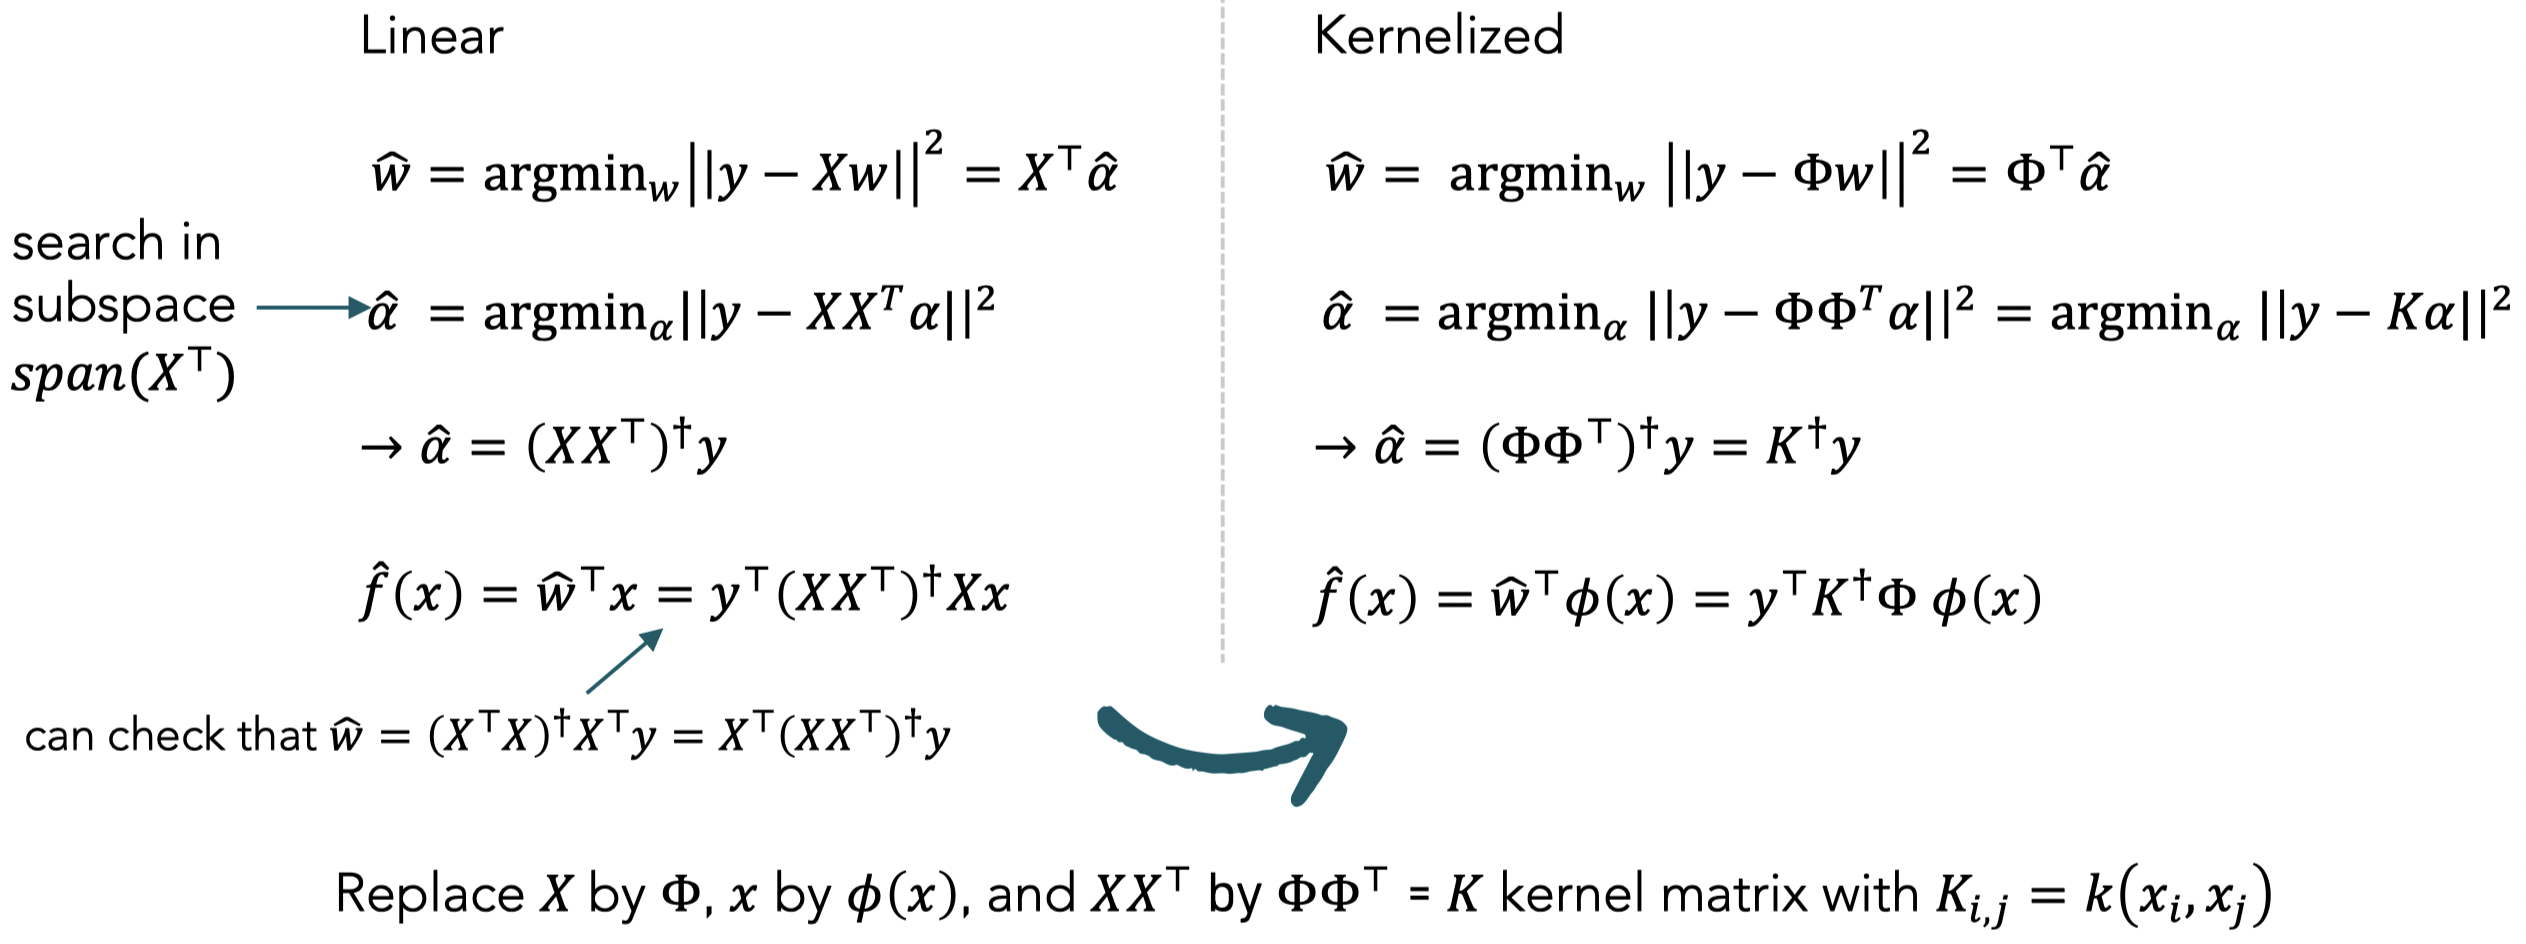
\includegraphics[width=15cm]{../images/IntroML_Fig5-1}
    \centering
\end{figure}

\begin{tbox}
    \textbf{Claim 2 (Representer Theorem):} The global minimizer(s) $\arg \min_{w \in \mathbb{R}^p} \frac{1}{n} \sum_{i = 1}^n l(y_i, \, w^T\phi(x_i)) + \lambda ||w||^2$ have the form $\hat{w} = \Phi^T\hat{\alpha}$ with some $\hat{\alpha} \in \mathbb{R}^n$, such that $\hat{f} = \sum_{i = 1}^n \hat{\alpha}_i \langle \phi(x_i), \, \phi(x) \rangle$.
\end{tbox}

Using the kernel trick, for ridge regression $\frac{1}{n}||y - \Phi w||^2 + \lambda ||w||^2$, using $w = \Phi^T\alpha$ and $K = \Phi \Phi^T$, we obtain
\[
    \frac{1}{n}||y - \Phi w||^2 + \lambda||w||^2 = \frac{1}{n}||y - \Phi \Phi^T \alpha ||^2 + \lambda || \Phi^T \alpha ||^2 = \frac{1}{n}||y - K \alpha ||^2 + \lambda \alpha^T K \alpha.
\]

\end{document}